\chapter{関連研究}
\label{chap:relatedResearch}

本章では関連研究を紹介し、それらの特徴や本研究との関連性について示す。

\newpage


\section{主要な研究領域}
本研究ではNFCのタッチインタラクション及びwikiベースなARナビゲーションが有用であることを検討した。
本研究に関連する先行研究は大きく以下のように分類できる
\begin{itemize}
  \item ARをナビゲーションに利用する研究
  \item AR情報の整理・関連情報推薦にハイパーリンクを利用する研究
  \item NFCをナビゲーションに利用した研究
\end{itemize}
それぞれについて関連性の高いものを紹介した上で本研究との関連性を示す。

\section{ARをナビゲーションに利用する研究}
ARを地理情報のナビゲーションとして利用する代表的な研究及びシステムを紹介する。

% \subsection{KARMA}
% FeinerらがKnowledge-based augmented reality\cite{10.1145/159544.159587}で提案したKARMA(図\ref{fig:karma})はレーザープリンターのメンテナンスをARで説明するプロトタイプシステムである。
% ヘッドマウント・ディスプレイによってレーザープリンターの内部機構に関する情報を提示しメンテナンスを助けるものであった。
% 位置測位は超音場センサを利用しておりこれらのセンサをすべての対象に取り付ける必要があるという難点があった。

% \begin{figure}[htbp]
%   \centering
%   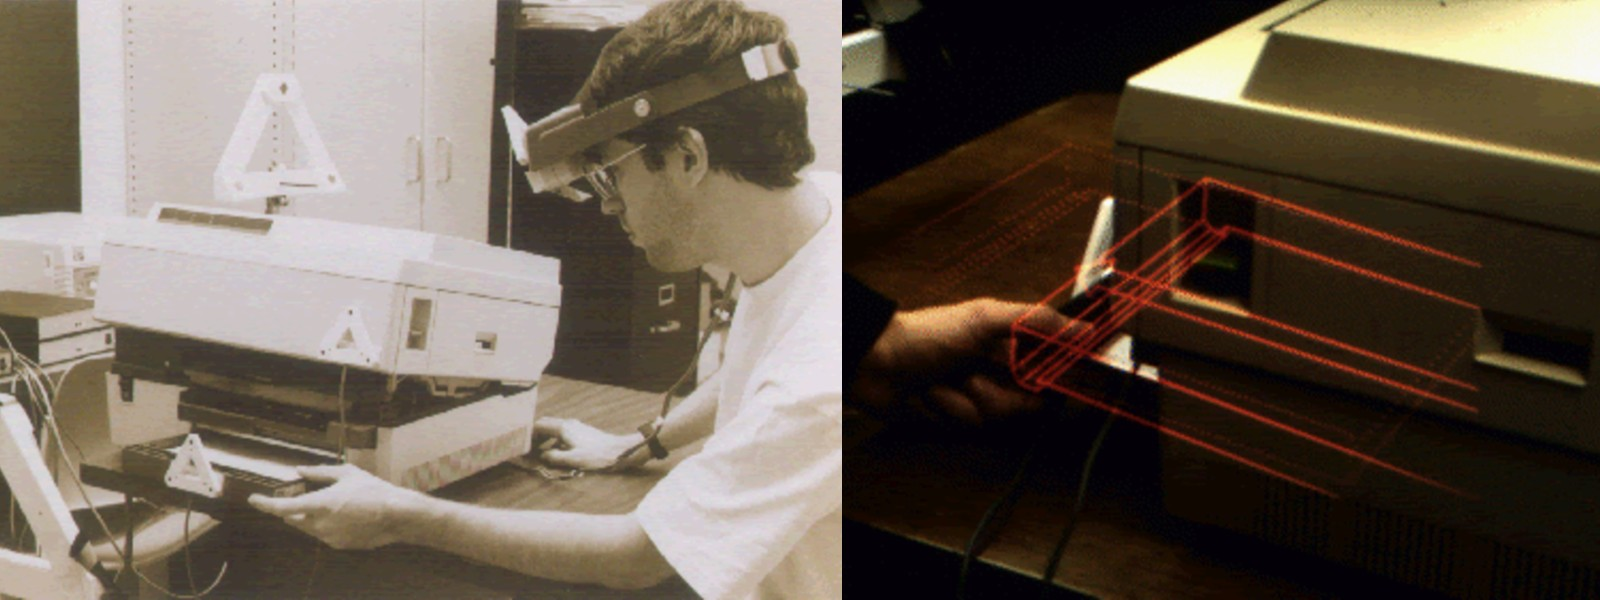
\includegraphics[width=150mm]{images/karma.jpg}
%   \caption{KARMA} \label{fig:karma}
% \end{figure}


\subsection{A Touring Machine}
Feinerらが開発したA Touring Machine\cite{629922}(図\ref{fig:a_touring_machine})はヘッドマウント・ディスプレイとスタライスで操作可能な2Dディスプレイで大学のキャンパスの情報を表示するアプリケーションである。
ARを利用した地理情報ナビゲーションの初期研究として挙げられる。
GPSによる位置情報と磁気センサによる向きの情報からユーザーの位置と向きを推定し、ヘッドマウント・ディスプレイに大学の情報が表示される。
また手持ちのスタライスで操作可能な2Dディスプレイが専用のHTTPサーバにつながっており、表示したい情報のリンクに触れるなどの操作することでヘッドマウント・ディスプレイでの表示情報が変化するようになっている。
一方でGPSと磁気センサによる位置推定には精度の面で課題があり、当時の技術ではヘッドマウント・ディスプレイとコンピュータを小型化することが難しかったため常用するには難しいものであった。

\begin{figure}[htbp]
  \centering 
  
\includegraphics[width=150mm]{images/wip.jpg}
  \caption{A Touring Machine} \label{fig:a_touring_machine}
\end{figure}


\subsection{Feature-Based Indoor Navigation Using Augmented Reality}
KasprzakらはFeature-Based Indoor Navigation Using Augmented Reality\cite{6597797}で室内での利用を想定したモバイル端末のARナビゲーションのプロトタイプを作成し評価している。
このプロトタイプは画像として登録された特徴的なアイコンなどを元に画像認識から位置情報と向きを推定し、ユーザーの目的地を矢印で表示するものである。
またこのプロトタイプを利用し、実際に建物内での案内に利用するテストを行っている。
その結果2Dの地図と比べて目的地までの到達時間が短縮され、被験者が立ち止まったり間違えた方向に進む回数も減少したと報告している。
室内での利用を視野に入れている点はGPSなどを利用するシステムと違い、本研究に近いが登録した画像による位置推定には以下のような課題もある。
\begin{itemize}
  \item 特徴的なロゴやアイコンの無いところでは登録できる画像がなく精度が保証できない
  \item 各場所で個別に画像の登録が必要
  \item 距離や明るさなどによっては認識できない可能性がある
\end{itemize}
またこのプロトタイプシステムでは事前に選択した目的地に正確に早く到着することに主眼を置いており、本システムのようにハイパーリンクによる関連情報から周辺譲歩を探索する用途を考えていない点も本研究との違いである。

\subsection{Wikitude}
Wikitude(図\ref{fig:Wikitude})は、Wikitude GmbH\footnote{\textsf{TODO:todo}}が開発したモバイル向けARソフトウェアである。
モバイル端末のGPSと磁気センサ、加速度計からユーザーの位置と向きを推測し周囲情報をディスプレイに表示する。
コンテンツの追加にはKMLやARML(Augmented Reality Markup Language)と呼ばれるXML互換のフォーマットが使われている。
KMLはGoogleMapなどが対応した地理空間情報の情報記述を目的としたXML互換のファイル形式であり、ARMLはKMLを更に拡張したファイル形式である。
KMLファイルはGoogleMapでの読み込みや作成が可能でありユーザーはGoogleMapからAR情報を作成できる。
一方でGPSと磁気センサによる位置推定には精度の面で課題があるだけでなく、GPSの利用できない屋内などでは利用できない欠点がある。
またARでの情報登録する際にGoogleMapなどの地図アプリケーションから作成するかKMLファイルを自身で編集する必要があり、本システムとは以下のような点で異なっている。
\begin{itemize}
  \item 共同編集が難しい
  \item 編集環境がWYSIWYGでない
  \item AR情報同士のハイパーリンクを記述するのが難しい
\end{itemize}


\section{AR・VR情報の整理・関連情報推薦にハイパーリンクを利用する研究}
ARやVRでの情報を整理するためにハイパーリンクを利用すた研究やプロジェクトを紹介する。

\subsection{VAnnotatoR}
Mehlerらが提案したVAnnotatoR\cite{10.1145/3209542.3209572}は

\subsection{Croquet Project}
Croquet Project\cite{10.1145/1152399.1152452}はKayらが主導した仮想OS構築プロジェクトであり、


\section{NFCをナビゲーションに利用した研究}
NFC技術を自己位置推定やコンテキスト情報取得などに利用し、ナビゲーションに役立てている研究を紹介する。

\subsection{Development of an Indoor Navigation System Using NFC Technology}
OzdenizciらはDevelopment of an Indoor Navigation System Using NFC Technology\cite{5954491}で